\section{Error versus performance}
\label{sec:errorvsperformance}

%Global H1 error as measure
%\begin{align}
%\| e_{hp} \|_{H^1(\Omega)}^2 &= \sum\limits_K \| e_{hp} (\vec{x}) \|_{H^1(K)}^2 \\
%\| e_{hp} \|_{H^1(K)}^2 &= \int_K (|e_{hp}|^2 + |\nabla e_{hp}|^2) \differential{\vec{x}}
%\end{align}
%with error function $e_{hp} = u - u_{hp}$.

% setup of scenario

The main motivation to use \hp-adaptive methods are their superior error convergence characteristics compared to the more common \h-adaptive methods, provided that the solution is sufficiently regular. We will demonstrate their advantages on our presented scenario and use consecutively adapted meshes to illustrate their error performance in relation to their workload on the numerical example.

%Demonstrate adaptive algorithms , and how the error reduces with.
%compare error with the workload either measured in the number of \glspl{dof} or the actual wall time. % maybe later

The consecutively adapted meshes so created are by far not optimal for the problem, nor is finding such an optimal mesh subject of this dissertation. We are rather interested in comparing the performance and results of the decision algorithms presented in Sec.~\ref{sec:decision}, and whether they are capable of localizing regions with singularities, i.e.\@ the one at the point of origin for our numerical example. We will compare all types of adaptation at our disposal, i.e.\@ \h-, \p-, and \hp-adaptation. For the latter, we examine all three presented strategies in contrast, namely error prediction and smoothness estimation by either Legendre or Fourier coefficient decay.

After solving the linear equation system in each step and calculating the error on basis of the analytic solution according to \textcite{kelly1983,davydov2017}, we use the \textit{fixed-number} strategy to indicate adaptation: The 30\% fraction of all cells with the highest error will be flagged for refinement, and 3\% of those with the lowest error will be marked for coarsening. This allows us to compare the results of each adaptation type under the same conditions, since always the same amount of cells is going to be changed. The idea behind additional coarsening is motivated by the fact that we tend to refine too many cells with error estimators providing an upper bound for the error, or error indicators based on heuristics. We would like to correct this from a previous iteration by coarsening a small amount of cells. The combination of fractions of 30\% for refinement and 3\% for coarsening has become a reasonable choice for two-dimensional applications within the \dealii{} library.

%We will compared different refinement strategies. We will use \textit{fixed-fraction} adaptation so that every cell is refined. This allows us to compare the choices of all strategies since always the same amount of cells is taken into account. \todo{see slack text}

Further for \hp-adaptive strategies, we need to choose a decision strategy providing corresponding indicators that propose which type of adaptation we want to impose on each cell.
%
Again, we use the \textit{fixed-number} algorithm on all decision indicators, as illustrated in Fig.~\ref{fig:indicators}. This allows us to compare the choices made by each strategy since always the same amount of cells is going to be changed in terms of both \h- and \p-adaptation, respectively.
%
As a first naive approach, we will impose the \h-variant on one half of all cells previously marked for adaptation, and the \p-variant on the other half.
%As a first naive approach, we choose between \h- and \p-adaptation fifty fifty among all cells that have been previously marked for adaptation.
%, based on the specified decision criterion.
As a second attempt, since we know that we have only one single localized and well-defined singularity in the domain, we are confident to make an educated guess and assign 90\% of flagged cells for \p- and the remaining 10\% for \h-adaptation. From here, we refer to the first approach if we call a decision strategy naive, and speak of the second if no such attribute was given.

To setup the numerical example, we start with a mesh consisting of three cells as the coarsest possible representation of our L-shaped domain, which will be globally refined five times to form the initial grid for all investigations in this section.

The error prediction strategy forms an exception since it requires a prepended initialization step. In this case, we will begin with four initial refinement steps, solve the equation system, and perform another global refinement so that we have the corresponding predicted errors available. Further for this strategy, control parameters are set to $\gamma_n = 1$, $\gamma_h = 1$, and $\gamma_p = \sqrt{0.4}$, which corresponds to the values used by \textcites{melenk2001}{mitchell2014}.

We use a collection of Lagrangian finite elements $Q_p$ with polynomial degrees $p \in [2,7]$ and thus skip linear elements due to our observation that the smoothness estimation algorithms perform poorly with those. All cells will be initially assigned with the lowest order element. In the case of sole \h-adaptation, all elements will be assigned to $Q_2$ elements. For pure \p-adaptation, we favor \p-adaptation over \h-adaptation as long as the finite element can be \p-adapted, i.e.\@ the current finite element is neither at the top nor the bottom of the hierarchy. We perform a total of twelve consecutive adaptation iterations, so twice as many as there are different finite elements.

All calculations in this section have been carried out on a desktop machine, using an Intel\textsuperscript{\textregistered} Core\textsuperscript{\texttrademark} i7-4790 processor running at 3.6 GHz with 32 GB of memory \todo{si units?}. Although this is a quad-core processor offering a total of eight threads utilizing hypertreading, we will only use a single thread for our calculations, which is sufficient to determine both error and workload. We will deal with parallelization in later sections.


% results: error vs ndofs

Representatively, we will show the grid and distribution of finite elements after six adaptation cycles of the Legendre coefficient decay strategy with the educated guess approach in Fig.~\ref{fig:fedegrees}. All other meshes after equally many adaptation iterations from the other strategies are showcased in App.~\ref{app::strategies}.

\todo{Add legend}
\begin{figure}
\centering
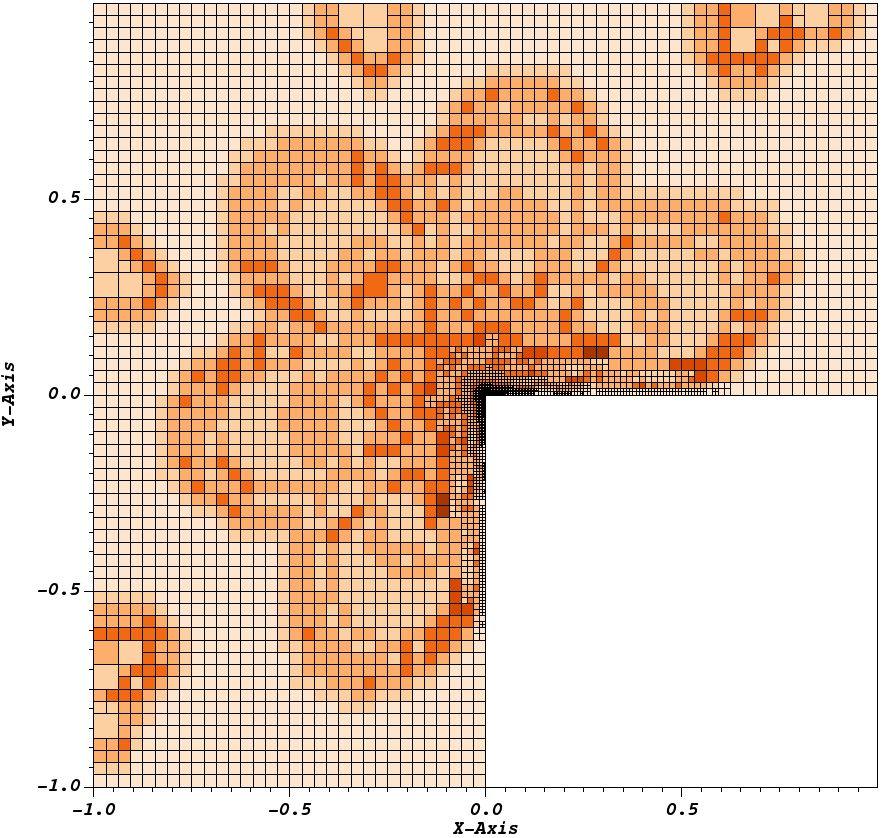
\includegraphics[width=0.49\textwidth]{figures/results/corner-2d-error-hp-legendre-05_fedegrees.png}
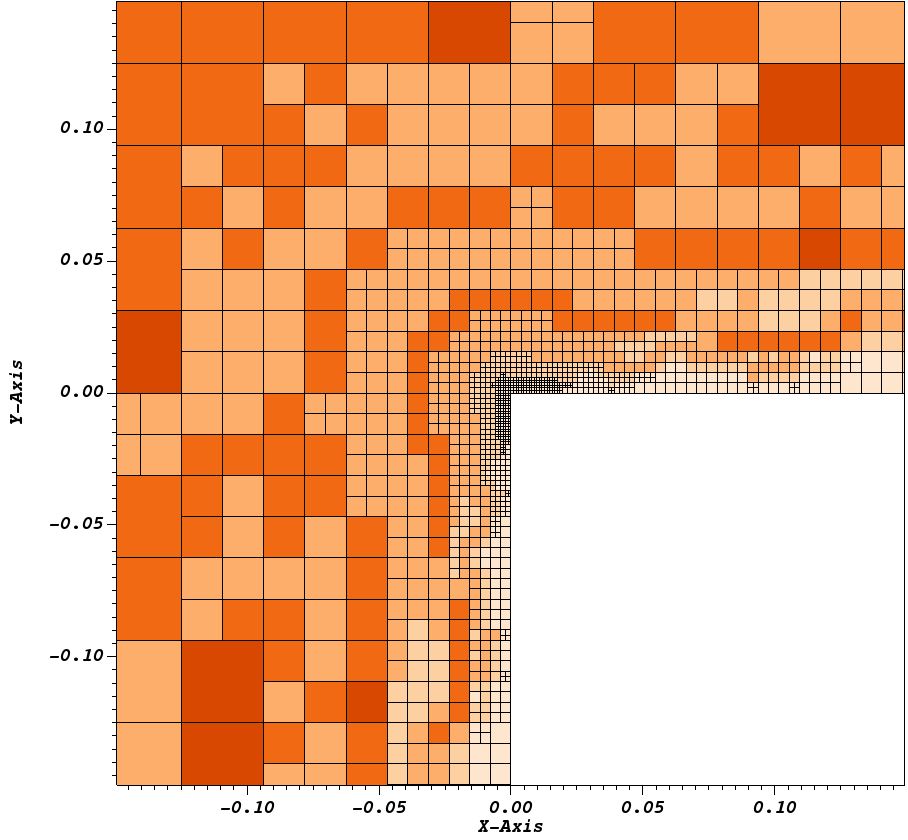
\includegraphics[width=0.49\textwidth]{figures/results/corner-2d-error-hp-legendre-05_fedegrees_zoom.png}
\caption{Distribution of finite elements after six iterations with the Legendre coefficient decay strategy.}
\label{fig:fedegrees}
\end{figure}

We see that the Legendre strategy is able to locate the singularity in the center by preferring \h-adaptive refinement in this section, while using \p-adaptation in the other regions. This is also the case for all other strategies, naiive or not, as shown in App.~\ref{app::strategies}.

We will plot the $H_1$-error against the workload, which can be measured in two ways: Either with the number of \glspl{dof}, or the elapsed real time from start to end of our application, which we call wall time. We begin with identifying the workload with the former and show corresponding results in Fig.~\ref{fig:errordofs}.

%We measure the workload in two different ways and present the results separately. First, with the number of \glspl{dof} for each individual iteration, and second, with the total wall time accumulated over the current and all previous iterations.

\begin{figure}
\begin{subfigure}{1\textwidth}
  \centering
  \begin{tikzpicture}
\begin{loglogaxis}[
  xlabel=Number of \glspl{dof},
  ylabel=H1 error]
\addplot table [y=H1 error, x=ndofs, col sep=comma] {data/error/h.csv};
\addplot table [y=H1 error, x=ndofs, col sep=comma] {data/error/p.csv};
\addplot table [y=H1 error, x=ndofs, col sep=comma] {data/error/hp-legendre.csv};
\addplot table [y=H1 error, x=ndofs, col sep=comma] {data/error/hp-fourier.csv};
\addplot table [y=H1 error, x=ndofs, col sep=comma] {data/error/hp-prediction.csv};
\addplot table [y=H1 error, x=ndofs, col sep=comma] {data/error/hp-legendre-naive.csv};
\addplot table [y=H1 error, x=ndofs, col sep=comma] {data/error/hp-fourier-naive.csv};
\addplot table [y=H1 error, x=ndofs, col sep=comma] {data/error/hp-prediction-naive.csv};
\end{loglogaxis}
\end{tikzpicture}%
  \caption{Double logarithmic representation. The thick line corresponds to the reference Eq.~(\ref{eq:errorbound_ana}).}
  \label{fig:errordofsloglog}
\end{subfigure}
\begin{subfigure}{1\textwidth}
  \centering
  \begin{tikzpicture}
\begin{semilogyaxis}[
%  scale only axis,
  xlabel=Number of \glspl{dof},
  ylabel=H1 error,
  legend pos=outer north east]
%\addplot table [y=H1 error, x=ndofs, col sep=comma] {data/error/h.csv};
%\addlegendentry{\h};

\addplot table [y=H1 error, x=ndofs, col sep=comma, select coords between index={0}{5}] {data/error/p.csv};
\addlegendentry{\p};

\addplot table [y=H1 error, x=ndofs, col sep=comma, select coords between index={0}{5}] {data/error/hp-legendre.csv};
\addlegendentry{\hp{}-Legendre};

\addplot table [y=H1 error, x=ndofs, col sep=comma, select coords between index={0}{5}] {data/error/hp-fourier.csv};
\addlegendentry{\hp{}-Fourier};

\addplot table [y=H1 error, x=ndofs, col sep=comma, select coords between index={0}{6}] {data/error/hp-prediction.csv};
\addlegendentry{\hp{}-prediction};

%\addplot table [y=H1 error, x=ndofs, col sep=comma] {data/error/hp-legendre-naive.csv};
%\addlegendentry{\hp{}-Legendre naive};
%
%\addplot table [y=H1 error, x=ndofs, col sep=comma] {data/error/hp-fourier-naive.csv};
%\addlegendentry{\hp{}-Fourier naive};
%
%\addplot table [y=H1 error, x=ndofs, col sep=comma] {data/error/hp-prediction-naive.csv};
%\addlegendentry{\hp{}-prediction naive};

%\addplot[very thick, samples=100, domain=10000:50000] {10^(-2)*exp(10^(-3.9)*(-x+10000))}; % {10^(-4)*(-x+10000)};
\end{semilogyaxis}
\end{tikzpicture}%
  \caption{Customly scaled coordinate system with the y-axis scaled exponentially and the x-axis scaled with the cubic root. The thick line corresponds to the reference Eq.~(\ref{eq:errorbound_exp}) with $b = 0.18$.}
  \label{fig:errordofscustom}
\end{subfigure}
\caption{Error performances of several adaptation strategies compared to their workload measured by the number of \glspl{dof}.}
\label{fig:errordofs}
\end{figure}

The double logarithmic representation of our results in Fig.~\ref{fig:errordofsloglog} reveals analytic convergence for the \h-adaptive case, but at a lower rate as presented in Eq.~(\ref{eq:errorbound_ana}), which translates to $n_\text{dofs}^{-1}$ in our scenario. An explanation would be that we are not working with quasiuniform but rather highly adapted meshes.

Eq.~(\ref{eq:errorbound_exp}) predicts exponential decay for \hp-adaptive strategies, which we would like to verify in Fig.~\ref{fig:errordofscustom} with a customly scaled plot featuring a logarithmic y-axis and an x-axis scaled with the cubic root, which corresponds to the correct exponent in our numerical example. Indeed, we see exponential convergence in the \p-adaptive and \hp-adaptive strategies to the proclaimed rate, however the naive approaches miss it. Thus a high proportion of \p-refinement is required to yield exponential decay in this scenario.

The \p-strategy shows a similar decay as the \hp-adaptive methods.
%, but the error in the last cycle is still by a factor of two higher.
In this strategy, \p-refinement will be applied up to the point until it is no longer possible after we reached the highest order element in the hierarchy. With six distinct finite elements in our collection, we will apply \h-refinement for the first time after the sixth data point, at which a major drop is observable. Therefore we conclude that the exponential decay proclaimed in Eq.~(\ref{eq:errorbound_exp}) is only observable after applying \h-refinement, which we thus consider mandatory to reduce the error to the observed low order of magnitude.

To solve the equation system in the last adaptation cycle, the \hp-adaptive methods %corresponding to our educated guess 
require a number of \glspl{dof} which is lower by a factor of 100 than the \h-adaptive methods to achieve the same accuracy
%need a factor of 1,000 less \gls{dof} to reach the same accuracy as the \h-adaptive methods
and by factor of 10 compared to their naive counterparts. This demonstrates that \hp-adaptive methods are the methods of choice for this particular scenario.

%We conclude that \p-heavy refinement combined with \h-adaptation near the singularity perform the best error per workload ratio.

In the course of adaptation with the Fourier strategy, some adaptation steps increase the number of \glspl{dof} without decreasing the error.
%, which we refer to as 'hickups'.
%We see certain outliers in the plots for Fourier strategy.
We observed that this occurs if the finite element with the highest polynomial degree in our mesh increases from fourth to fifth order. This is perhaps not a causal relation, and we have not yet found the reason for this behavior.

%Compared to \h- and naive \hp-approaches, \p- and \hp-strategies featuring the educated guess yield similar results.

%We reach about one order of magnitude lower errors with \hp-adaptive strategies compared to the \p-adaptive, which might be due to the singularity that the latter does not resolve \todo{?}.


% results: error vs walltime

From a practical point of view, the error performance will now be compared to the actual wall time to measure whether we have an economic benefit in using \hp-adaptive methods. For each consecutive adaptation cycle, we again plot the calculated error against the workload, which is this time represented by the total run time accumulated over the current and all previous iterations. Each run will be repeated five times and the minimum over the total runtime over all runs will be picked to compensate for temporarily high loads on memory bandwidth. The results are shown in Fig.~\ref{fig:errorwalltime}.

\begin{figure}
%\begin{subfigure}{1\textwidth}
\centering
\begin{tikzpicture}
\begin{loglogaxis}[
  xlabel=Wall time {[seconds]},
  ylabel=H1 error,
  legend pos=outer north east]
\addplot table [y=H1 error, x=walltime, col sep=comma] {data/error/h.csv};
\addlegendentry{\h};

\addplot table [y=H1 error, x=walltime, col sep=comma] {data/error/p.csv};
\addlegendentry{\p};

\addplot table [y=H1 error, x=walltime, col sep=comma] {data/error/hp-legendre.csv};
\addlegendentry{\hp{}-Legendre};

\addplot table [y=H1 error, x=walltime, col sep=comma] {data/error/hp-fourier.csv};
\addlegendentry{\hp{}-Fourier};

\addplot table [y=H1 error, x=walltime, col sep=comma] {data/error/hp-prediction.csv};
\addlegendentry{\hp{}-prediction};

\addplot table [y=H1 error, x=walltime, col sep=comma] {data/error/hp-legendre-naive.csv};
\addlegendentry{\hp{}-Legendre naive};

\addplot table [y=H1 error, x=walltime, col sep=comma] {data/error/hp-fourier-naive.csv};
\addlegendentry{\hp{}-Fourier naive};

\addplot table [y=H1 error, x=walltime, col sep=comma] {data/error/hp-prediction-naive.csv};
\addlegendentry{\hp{}-prediction naive};
\end{loglogaxis}
\end{tikzpicture}%
%  \caption{Error vs workload.}
%  \label{fig:errorexpworkload}
%\end{subfigure}
%\begin{subfigure}{1\textwidth}
%  \centering
%  \begin{tikzpicture}
\begin{semilogyaxis}[
  xlabel=Wall time {[seconds]},
  ylabel=H1 error,
  legend pos=outer north east]
%\addplot table [y=H1 error, x=walltime, col sep=comma] {data/error/h.csv};
%\addlegendentry{\h};

\addplot table [y=H1 error, x=walltime, col sep=comma, select coords between index={0}{5}] {data/error/p.csv};
\addlegendentry{\p};

\addplot table [y=H1 error, x=walltime, col sep=comma, select coords between index={0}{5}] {data/error/hp-legendre.csv};
\addlegendentry{\hp{}-Legendre};

\addplot table [y=H1 error, x=walltime, col sep=comma, select coords between index={0}{5}] {data/error/hp-fourier.csv};
\addlegendentry{\hp{}-Fourier};

\addplot table [y=H1 error, x=walltime, col sep=comma, select coords between index={0}{6}] {data/error/hp-prediction.csv};
\addlegendentry{\hp{}-prediction};

%\addplot table [y=H1 error, x=walltime, col sep=comma] {data/error/hp-legendre-naive.csv};
%\addlegendentry{\hp{}-Legendre naive};
%
%\addplot table [y=H1 error, x=walltime, col sep=comma] {data/error/hp-fourier-naive.csv};
%\addlegendentry{\hp{}-Fourier naive};
%
%\addplot table [y=H1 error, x=walltime, col sep=comma] {data/error/hp-prediction-naive.csv};
%\addlegendentry{\hp{}-prediction naive};

%\addplot[very thick, samples=100, domain=0.1:5] {10^(-2)*exp(10^(0)*(-x+0.1))}; % {10^(-4)*(-x+10000)};
\end{semilogyaxis}
\end{tikzpicture}
%  \caption{Error vs walltime.}
%  \label{fig:errorexpwalltime}
%\end{subfigure}
\caption{Double lagarithmic representation of error performances of several adaptation strategies compared to their workload measured by the wall time.}
\label{fig:errorwalltime}
\end{figure}

%We notice that the choice of the \hp-adaptive strategy has an impact on the error performance compared to the number of \glspl{dof}. However in comparing error with the runtime, we see that all methods perform similarly. We will postpone the discussion on this topic for the later Sec.~() in which we give an in-depth analysis on the sacalability of certain parts of our code, in which we think to identify the reason for this behavior.

Again after the last adaptation cycle, \p- and \hp-adaptive methods are about an order of magnitude faster than the \h-adaptive variant and thus the most efficient. Interestingly, the wall times of the naive \hp-strategies fan out. It appears that a high diversity of finite elements compared with major grid adaptation increases the wall time significantly, and we suspect that the combination of solver and \gls{amg} preconditioner is responsible for this behavior. We will discuss our choice of the preconditioner later in the scalability analysis.

The Fourier strategy takes the longest wall time for initialization, during which the Fourier transformation matrices are calculated. This is a costly operation, which requires substantially more quadrature points during calculation than the Legendre equivalent, and is responsible for the observable offset.

% this is general observation
Among all \hp-strategies of either naive or educated guess category, we do not see major differences in their performance, but overall the Legendre coefficient decay strategy stands out in both categories with the best error per workload performance in either way workload is defined.
%Compared to the Fourier strategy, it seems to be better suited for \gls{fem} since its basis functions are also based on polynomials.

Note that the results presented in this section are specific for our numerical example, in which the solution is sufficiently smooth over the entire domain except for the singularity at the origin. The error performance might differ if the presented techniques will be applied to a different scenario.

% write this in the next chaper
%In the upcoming scalability analysis, we will thus pick this strategy with Legendre coefficient and the educated guess.

%Overall, the Legendre coefficient strategy yields the best error per workload performance in both categories.

%Again, to mitigate the impact of temporary slowdowns on the supercomputer due to a high loads on memory and network bandwidth, we repeat each run for a total of \todo{five?} times and take the minimal runtime in each category over all runs.